\documentclass{beamer}
\usetheme{Madrid}
\usecolortheme{default}
\usepackage{tikz}
\usepackage{algorithm}
\usepackage{algpseudocode}
\usepackage{amsmath}
\usetikzlibrary{calc, positioning, arrows.meta}
\title[LLM-LNS for MILP]{Large Language Model-driven Large Neighborhood Search for Large-Scale MILP Problems}
\author[Ye et al.]{Huigen Ye, Hua Xu, An Yan, Yaoyang Cheng}
\institute[]{Tsinghua University}
\date{ICML 2025}

\begin{document}
	
	% Slide 1: Title
	\begin{frame}
		\titlepage
	\end{frame}
	
	% Slide 2: Motivation and Background
	\begin{frame}{Background: MILP and LNS}
		\begin{itemize}
			\item \textbf{Mixed Integer Linear Programming (MILP)} is a versatile framework for complex optimization, but it is NP-hard[cite: 2026, 2031].
			\item Exact algorithms (e.g., branch-and-bound) struggle with the computational demands of large-scale instances[cite: 2033].
			\item \textbf{Large Neighborhood Search (LNS)} is a popular heuristic that iteratively improves solutions by destroying and repairing parts of them[cite: 2034].
			\item \textbf{The Bottleneck:} LNS performance heavily depends on neighborhood selection, which traditionally requires labor-intensive expert knowledge[cite: 2035].
		\end{itemize}
	\end{frame}
	
	% Slide 3: Challenges with Current ML Approaches
	\begin{frame}{Limitations of Existing ML-based LNS}
		Machine learning has been applied to automate neighborhood selection, but faces challenges[cite: 2037]:
		\vspace{0.5cm}
		\begin{itemize}
			\item \textbf{Reinforcement Learning (RL):} Suffers from slow convergence in large-scale MILPs due to the vast search space[cite: 2039].
			\item \textbf{Imitation Learning:} Requires massive amounts of high-quality, labeled data, which is computationally expensive to generate[cite: 2040].
			\item \textbf{Existing LLM approaches (e.g., FunSearch, EOH):} Rely on fixed evolutionary strategies, limiting solution diversity and leading to premature convergence[cite: 2049, 2112].
		\end{itemize}
	\end{frame}
	
	% Slide 4: Proposed Framework Overview
	\begin{frame}{Proposed Solution: LLM-LNS}
		\textbf{LLM-LNS} is a novel LLM-driven LNS framework designed to automate and optimize neighborhood selection for large-scale MILP problems[cite: 2019, 2020].
		
		\vspace{0.3cm}
		\textbf{Key Innovations:}
		\begin{enumerate}
			\item \textbf{Dual-layer Self-evolutionary LLM Agent:} Automates heuristic generation by evolving both strategies and prompts[cite: 2053].
			\item \textbf{Differential Memory for Directional Evolution:} Guides crossover and variation operations to accelerate convergence[cite: 2055, 2056].
			\item \textbf{Adaptive Large Neighborhood Search (ALNS):} Dynamically adjusts search space size based on real-time LLM evaluations[cite: 2268].
		\end{enumerate}
	\end{frame}
	
	% Slide 5: Dual-Layer Agent - Inner Layer
	\begin{frame}{Dual-Layer Agent: Inner Layer (Heuristic Evolution)}
		The \textbf{Inner Layer} focuses on evolving heuristic strategies (thoughts and code) to ensure rapid convergence[cite: 2054, 2162].
		
		\begin{itemize}
			\item \textbf{Initialization:} Generates initial heuristics based on problem structure and initial prompts[cite: 2164].
			\item \textbf{Evolution:} Parent strategies are selected based on fitness and combined with evolutionary prompts to generate offspring[cite: 2166, 2168].
			\item \textbf{Evaluation:} Heuristics are tested on small-scale training instances to calculate their fitness (objective value improvements)[cite: 2170, 2171].
		\end{itemize}
	\end{frame}
	
 

		\begin{frame}{Inner Exploitation Loop:  Evolution of Heuristics}
			\vskip -2mm
		 Exploitation: find the best possible heuristics with  evolution prompt fixed
		 \vskip 3mm
			\centering
			% Resize the diagram to exactly the width of the slide text area
			% The '!' tells LaTeX to keep the aspect ratio the same
			\resizebox{\textwidth}{!}{%
				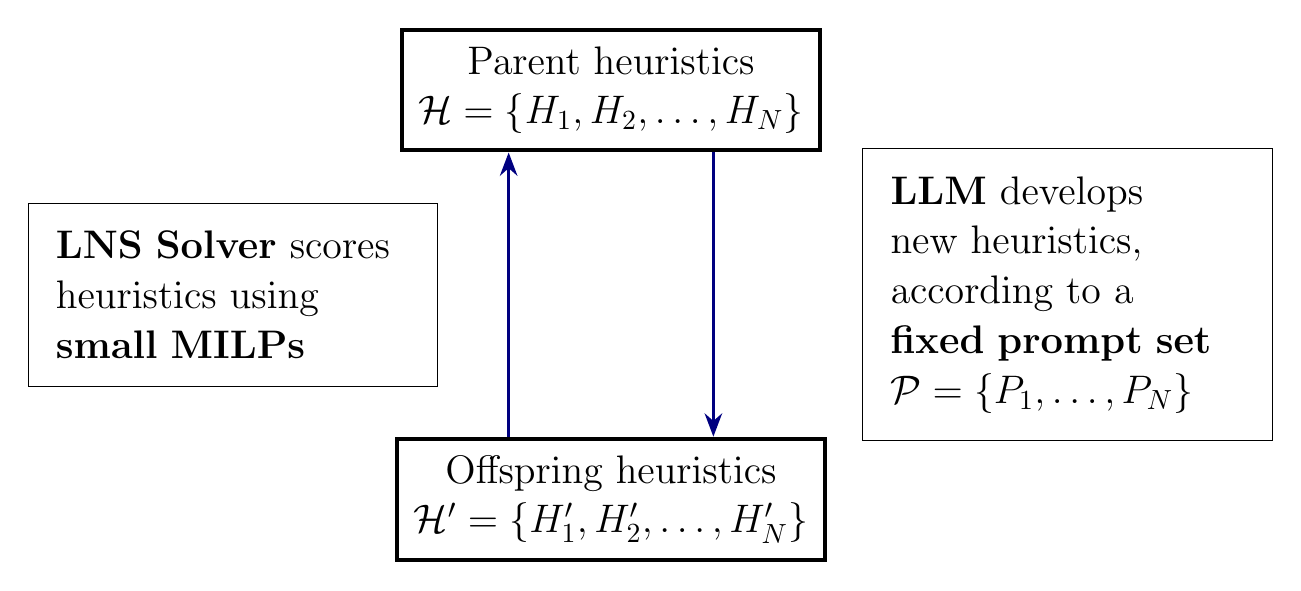
\begin{tikzpicture}[
					centerbox/.style={
						draw,
						rectangle,
						align=center,
						inner sep=6pt,
						line width=1.5pt,
						font=\Large
					},
					sidebox/.style={
						draw,
						rectangle,
						align=left,
						inner sep=10pt,
						text width=4.5cm,
						font=\Large
					}
					]
					
					% Main boxes
					\node (parent) [centerbox] at (0, 2.6) {Parent heuristics \\ $\mathcal{H}  = \{ H_1, H_2, \ldots, H_N \}$};
					\node (offspring) [centerbox] at (0, -2.6) {Offspring heuristics \\ $\mathcal{H}' = \{ H_1', H_2', \ldots, H_N' \}$};
					
					% Left/Right boxes 
					\node (solver) [sidebox] at (-4.8, 0) {\textbf{LNS Solver} scores heuristics using \textbf{small MILPs}};
					\node (llm) [sidebox] at (5.8, 0) {\textbf{LLM} develops new heuristics, according to a \textbf{fixed prompt set} $\mathcal{P} = \{P_1, \ldots, P_N\}$};
					
					% Arrows 
					\draw [-{Stealth}, line width=1.2pt, color=blue!50!black] 
					($(offspring.north)-(1.3cm, 0)$) -- ($(parent.south)-(1.3cm, 0)$);
					\draw [-{Stealth}, line width=1.2pt, color=blue!50!black] 
					($(parent.south)+(1.3cm, 0)$) -- ($(offspring.north)+(1.3cm, 0)$);
					
				\end{tikzpicture}%
			} 
	Repeat   for a fixed number of time; the whole procedure can be written as 
\begin{equation*}
	\mathcal{H}= \texttt{inner}(\texttt{prompt})
\end{equation*}		
			% End of resizebox
		\end{frame}
		

\begin{frame}
	\begin{itemize}
		\item Generation 0: capacity ratio with penalties
		\begin{equation*}
			\text{scores}[\text{bins} > \text{item}] = \frac{\text{bins} - \text{item}}{\text{bins}} \times \frac{1}{\text{index of bin} + 0.5} 
		\end{equation*}
		
		\item Generation 5:  Random exploration factor added
		\begin{align*}
			\text{scores}[\text{bins} > \text{item}] &= \frac{\text{bins} - \text{item}}{\text{bins} + 10^{-5}} - \frac{
				\frac{\text{bins}^2}{10^2}
			}{
				\max\left(\frac{\text{bins}^2}{10^2}\right)
			} \left( 1 - \frac{\text{bins} - \text{item}}{\max(\text{bins})} \right) 
			\\& \quad + \text{randomness} \times 0.1 
		\end{align*}
		
		\item Generation 8: Advanced hybrid optimization methods, such as genetic algorithms combined with tabu search, are introduced
		\begin{align*}
			\text{scores}[\text{bins} > \text{item}] &= \frac{\text{bins} - \text{item}}{\text{bins} + 10^{-5}} - \text{history penalty} - \frac{
				\frac{\text{bins}^2}{15^2}
			}{\max\left(\frac{\text{bins}^2}{15^2}\right)} 
			\\& \quad + \text{mutation variance} - \left( 1 - \frac{\text{bins} - \text{item}}{\max(\text{bins}) + 10^{-5}} \right) 
		\end{align*}
	\end{itemize}
\end{frame}
\begin{frame}{Outer Exploration Loop: Evolution of Prompts}
	\vskip -2mm
	Exploration: when inner loop stagnates, change the prompt
	\vskip 3mm
	\centering
	
	% Added [H] here to prevent Beamer floating errors
	\begin{algorithm}[H]
		\caption{Outer loop for exploration}
		\begin{algorithmic}[1] % [1] enables line numbering
			\Require Initial heuristic $H_0$, Initial prompt $P$, Total iterations $T$
			\For{$t = 1$ \textbf{to} $T$}
			\State $\mathcal{H}_{t} \gets \text{inner}(P)$
			\If{no improvement of $\mathcal{H}_{t}$ for a certain number of steps}
			\State $P \gets \texttt{LLMevolve}(P)$
			\EndIf
			\EndFor
		\end{algorithmic}
	\end{algorithm}
	
Final step: use the best strategy out of $\mathcal{H}_T$ and run LNS on massive MILP.	
\end{frame}

\begin{frame}
	\begin{itemize}
		\item \textbf{Generation 1: Initialization by handcrafted prompts}   ``Create a completely new algorithm'', ``Modify the given algorithm'' 
		
		\item \textbf{Generation 6: Addressing Stagnation.} ``Reconfigure heuristic principles to \textbf{reduce computational complexity} while maintaining effectiveness.'' 

		
		\item \textbf{Generation 10: Stochastic Adjustment.}  ``Enhance diversity by \textbf{introducing stochastic elements} to refine exploration strategies.'' 

 
	\end{itemize}
\end{frame}
	% Slide 7: Differential Memory
\begin{frame}{Inside the LLM: Differential Memory for Directional Evolution}
	\begin{itemize}
		\item \textbf{Historical Context:} Inside the inner loop, LLM reads a set of $m$ strategy-thought-fitness tuples, capturing both successful and unsuccessful heuristics:
		$$S^{(t)} = \left\{ \langle H_i^{(t)}, \text{thought}_i, f(H_i^{(t)}) \rangle \right\}_{i=1}^m$$
		
		\item \textbf{Directional Evolution:} The model $M$ generates the next iteration by conditioning on this historical memory:
		$$H_i^{(t+1)} = \texttt{LLM}(p_{\text{meta}} \parallel S^{(t)})$$
		
		\item \textbf{The Meta-Prompt ($p_{\text{meta}}$):} Combines two key components:
		\begin{itemize}
			\item[--] The strategic prompt provided by the Outer Loop.
			\item[--] A differential memory instruction: \textit{``Learn from history, both good and bad. Think of what makes the difference.''}
		\end{itemize}
	\end{itemize}
\end{frame}
	
	% Slide 8: Integration with ALNS
	\begin{frame}{Integration: Adaptive Large Neighborhood Search}
		The best evolved heuristic is seamlessly integrated into an ALNS framework[cite: 2268, 2578].
		
		\begin{itemize}
			\item \textbf{Variable Scoring:} The LLM-generated heuristic scores decision variables based on their potential to improve the objective value[cite: 2269].
			\item \textbf{Dynamic Resizing:} 
			\begin{itemize}
				\item If improvements plateau, the neighborhood size expands to search a broader space[cite: 2276].
				\item If subproblem solving takes too long, the neighborhood size shrinks to maintain efficiency[cite: 2277].
			\end{itemize}
			\item \textbf{Generalization:} Strategies trained on small-scale problems easily transfer to large-scale testing datasets[cite: 2280].
		\end{itemize}
	\end{frame}
	
	% Slide 9: Experimental Setup
	\begin{frame}{Experimental Setup}
		\textbf{Task 1: Combinatorial Optimization} [cite: 2290]
		\begin{itemize}
			\item Problems: Online Bin Packing, Traveling Salesman Problem (TSP)[cite: 2291].
			\item Baselines: Hand-crafted heuristics, Neural Networks (POMO, LEHD), and LLM-based approaches (FunSearch, EOH)[cite: 2304, 2313].
		\end{itemize}
		
		\vspace{0.3cm}
		\textbf{Task 2: Large-Scale MILP Benchmark} [cite: 2322, 2323]
		\begin{itemize}
			\item Datasets: Set Covering (SC), Minimum Vertex Cover (MVC), Maximum Independent Set (MIS), Mixed Integer Knapsack Set (MIKS)[cite: 2323, 2330].
			\item Trained on instances with $\sim 10K$ variables, tested on instances with up to $1$ Million variables[cite: 2331, 2846].
			\item Baselines: ACP, CL-LNS, Gurobi, SCIP, GNN\&GBDT, Light-MILPOPT[cite: 2332, 2333].
		\end{itemize}
	\end{frame}
	
	% Slide 10: Results - Combinatorial Optimization
	\begin{frame}{Results: Combinatorial Optimization}
		LLM-LNS outperforms both traditional and state-of-the-art LLM methods in heuristic generation tasks[cite: 2286].
		
		\begin{itemize}
			\item \textbf{Online Bin Packing:} Achieved an average excess bin fraction of 1.63\%, significantly outperforming FunSearch (2.31\%) and EOH (2.09\%)[cite: 2305].
			\item \textbf{TSP:} Achieved the lowest average gap to best-known solutions (0.08\%), beating advanced ML methods and EOH (0.16\%)[cite: 2315].
			\item \textbf{Efficiency:} Achieved these results using the same computational limits and population sizes as EOH, proving the superior efficiency of the dual-layer architecture[cite: 2318, 2319].
		\end{itemize}
	\end{frame}
	
	% Slide 11: Results - Large-Scale MILP
	\begin{frame}{Results: Large-Scale MILP Generalization}
		LLM-LNS successfully generalizes from small training data to massive test instances[cite: 2331, 2428].
		
		\begin{itemize}
			\item \textbf{Superior Objective Values:} Consistently found better solutions across large-scale instances compared to traditional solvers (Gurobi, SCIP) and ML frameworks[cite: 2341, 2348].
			\item \textbf{Faster Convergence:} Reaches high-quality solutions much earlier in the optimization process than all baselines[cite: 2356].
			\item \textbf{Primal Integral:} Achieved over a 20\% improvement in the primal integral compared to the closest competitor on massive datasets like $SC_2$ and $MVC_2$[cite: 2416].
		\end{itemize}
	\end{frame}
	
	% Slide 12: Conclusion
	\begin{frame}{Conclusion}
		\begin{itemize}
			\item \textbf{LLM-LNS} is a highly effective framework that bridges Large Language Models with operations research for solving massive MILP problems[cite: 2019, 2051].
			\item The \textbf{Dual-layer Self-evolutionary LLM Agent} perfectly balances exploitation (inner layer) and exploration (outer layer)[cite: 2122, 2161].
			\item \textbf{Differential Memory} allows the LLM to learn directional improvements rather than relying on blind mutations[cite: 2246, 2248].
			\item The framework requires minimal small-scale training data to produce highly scalable heuristic algorithms capable of beating commercial solvers on large benchmarks[cite: 2020, 2426, 2428].
		\end{itemize}
		\vspace{0.5cm}
		\begin{center}
			\textbf{Thank You!}
		\end{center}
	\end{frame}
	
\end{document}